% Scale Diffusion for Molecular Generation & Multifunctional Coating AI Platform
% Compile with: pdflatex mindmap.tex
\documentclass[border=15mm]{standalone}

\usepackage[T1]{fontenc}
\usepackage{lmodern}
\usepackage{tikz}
\usetikzlibrary{mindmap,backgrounds,positioning}

% Colour palette
\definecolor{coreGray}{HTML}{495057}
\definecolor{brTheory}{HTML}{1971C2}
\definecolor{brMolSS}{HTML}{2F9E44}
\definecolor{brArch}{HTML}{9C36B5}
\definecolor{brCoat}{HTML}{E8590C}
\definecolor{brPlatform}{HTML}{0CA678}
\definecolor{brData}{HTML}{D6336C}
\definecolor{brValid}{HTML}{4263EB}

\begin{document}
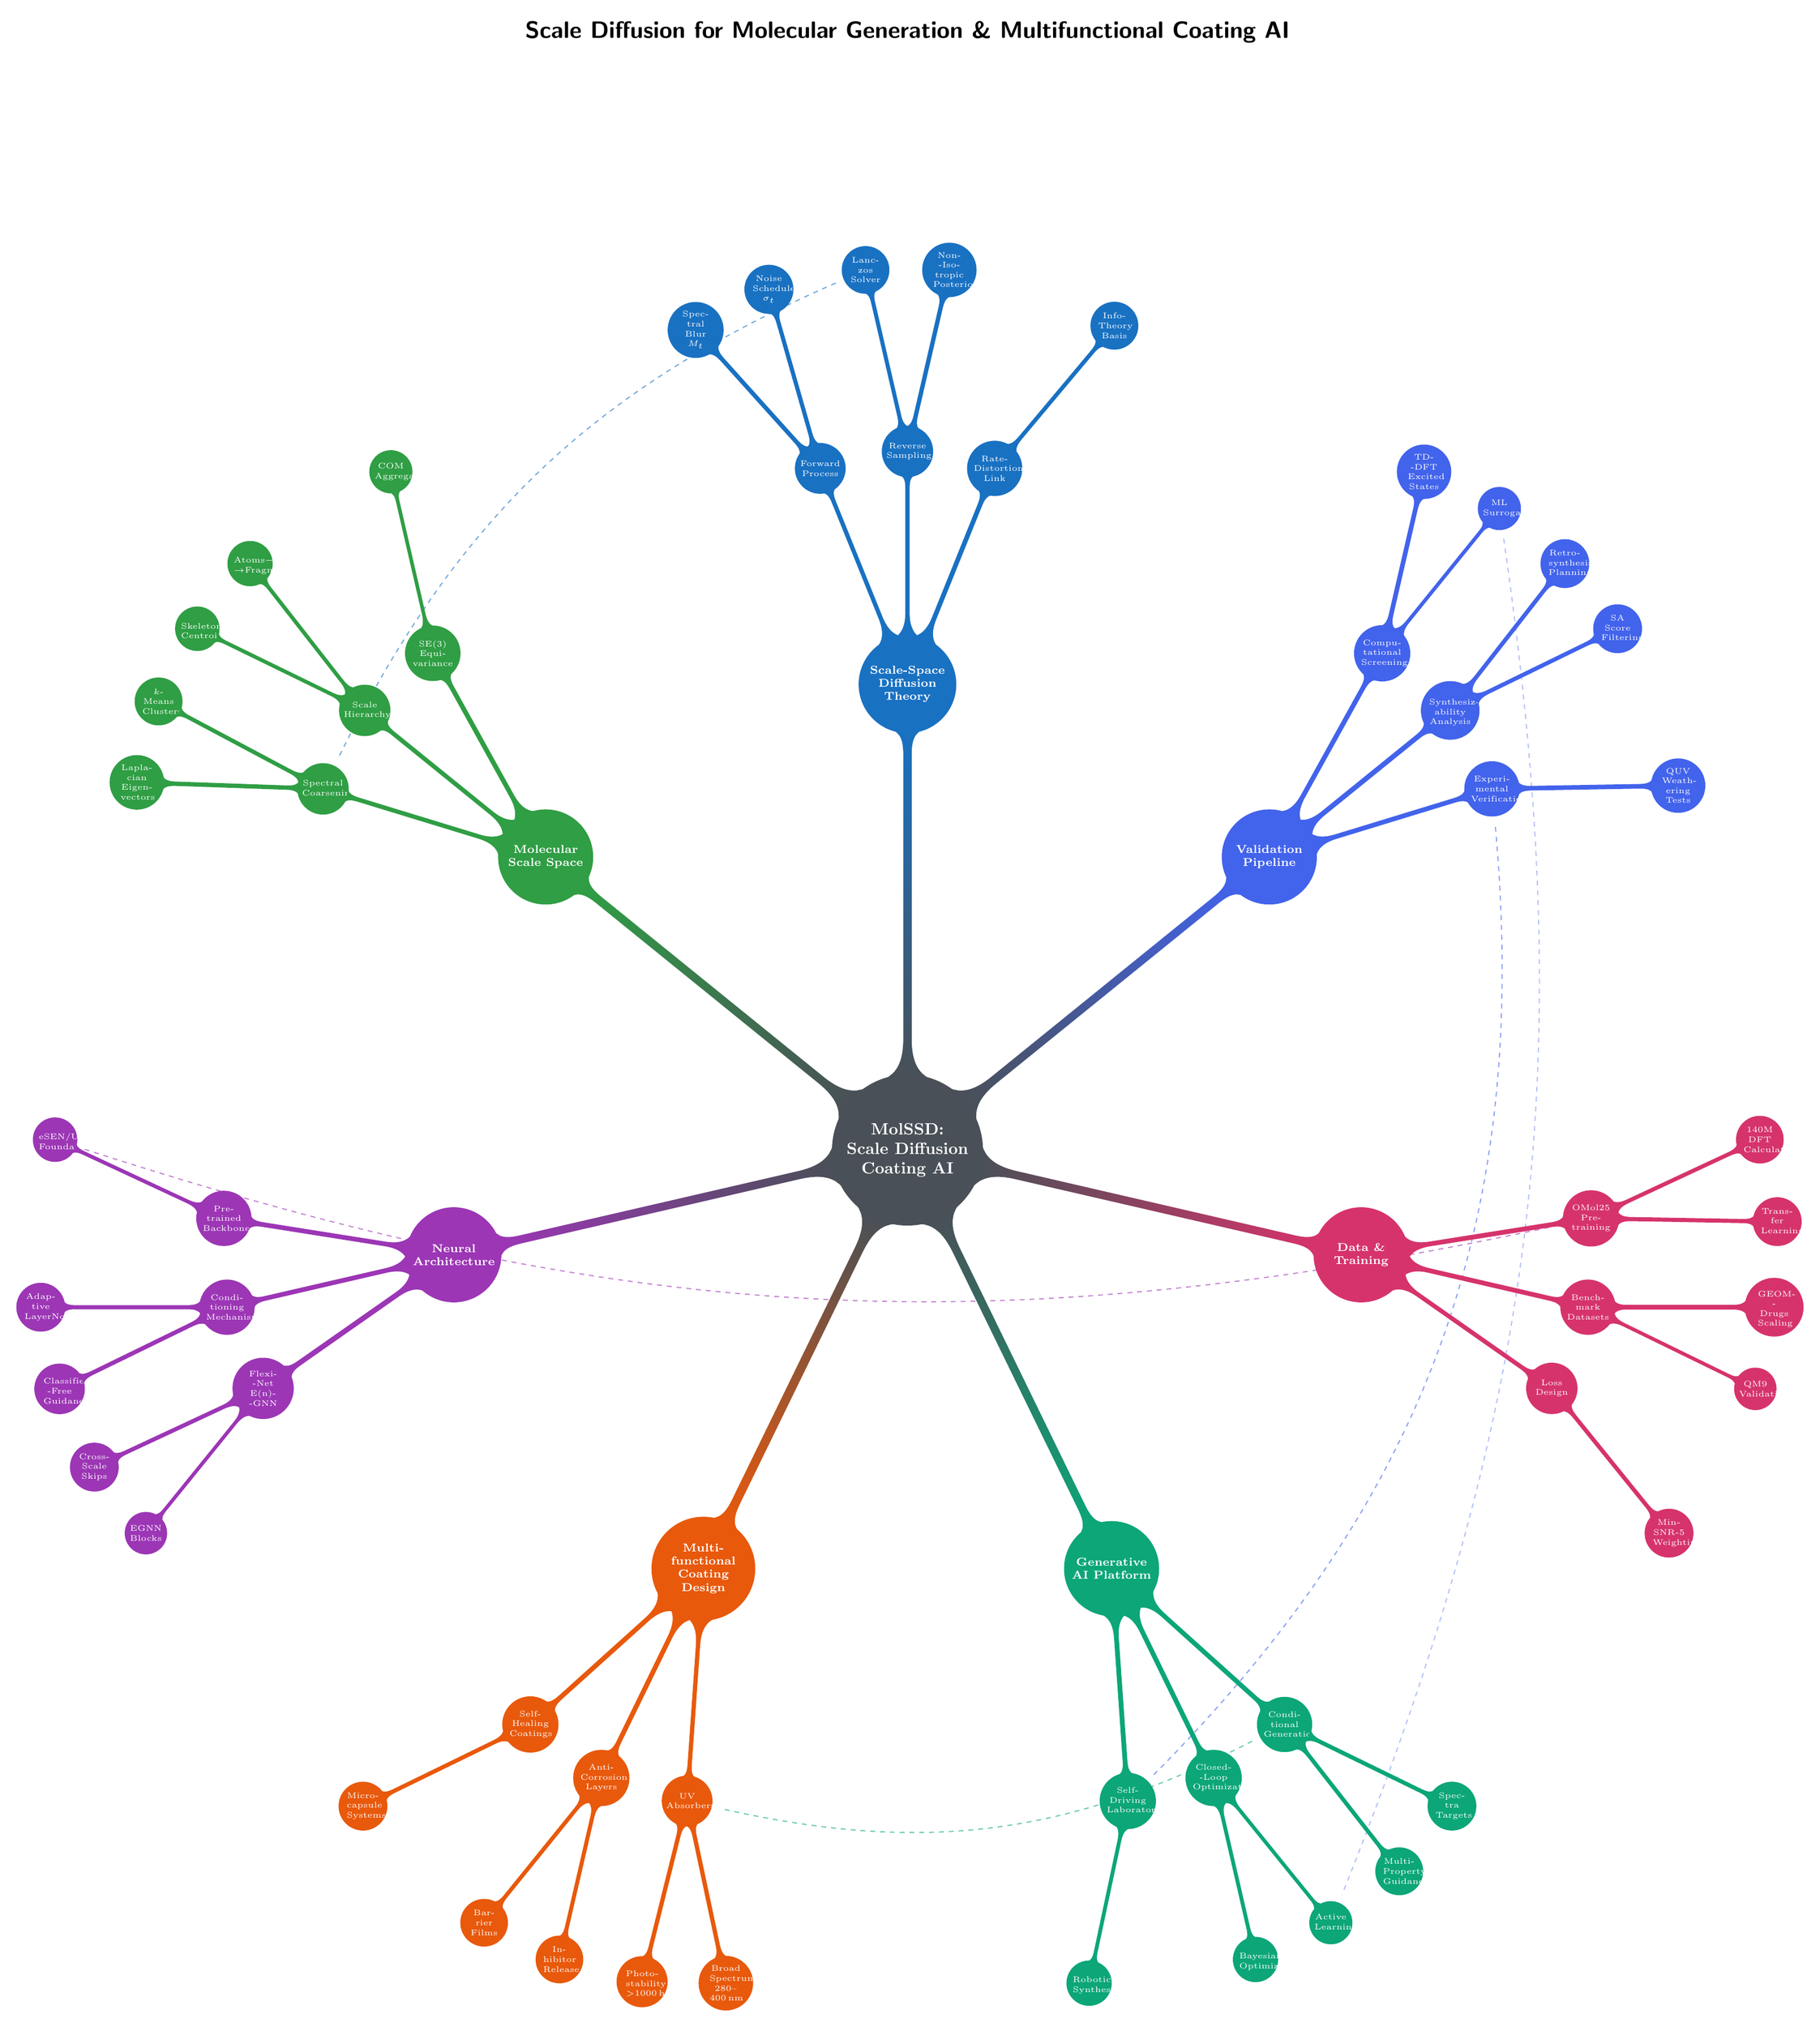
\begin{tikzpicture}

% Title
\node[font=\Large\bfseries\sffamily] at (0,24)
  {Scale Diffusion for Molecular Generation \& Multifunctional Coating AI};

\begin{scope}[
  mindmap,
  every node/.style={concept, execute at begin node=\hskip0pt},
  grow cyclic,
  text=white,
  concept color=coreGray,
  level 1/.append style={
    level distance=10cm, sibling angle=51,
    font=\scriptsize\bfseries, minimum size=2.0cm, text width=1.8cm,
  },
  level 2/.append style={
    level distance=5.0cm, sibling angle=22,
    font=\tiny, minimum size=1.0cm, text width=0.9cm,
  },
  level 3/.append style={
    level distance=4.0cm, sibling angle=26,
    font=\tiny, minimum size=0.8cm, text width=0.7cm,
  },
]

\node [font=\normalsize\bfseries, minimum size=3.2cm, text width=2.8cm]
  {MolSSD:\\Scale Diffusion\\Coating AI}
  %
  %% === Branch 1: Scale-Space Diffusion Theory (grow=90, blue) ===
  child [concept color=brTheory, grow=90] {
    node {Scale\--Space\\Diffusion\\Theory}
    child [grow=112] {
      node {Forward\\Process}
      child [grow=132] { node {Spectral\\Blur $M_t$} }
      child [grow=106] { node {Noise\\Schedule $\sigma_t$} }
    }
    child [grow=90] {
      node (reversesamp) {Reverse\\Sampling}
      child [grow=77] { node {Non\--Iso\-tropic\\Posterior} }
      child [grow=103] { node (lanczos) {Lanczos\\Solver} }
    }
    child [grow=68] {
      node {Rate\--Distortion\\Link}
      child [grow=50] { node {Info\--Theory\\Basis} }
    }
  }
  %
  %% === Branch 2: Molecular Scale Space (grow=141, green) ===
  child [concept color=brMolSS, grow=141] {
    node {Molecular\\Scale Space}
    child [grow=163] {
      node (speccoarse) {Spectral\\Coarsening}
      child [grow=178] { node {Laplacian\\Eigen\-vectors} }
      child [grow=152] { node {$k$\--Means\\Clusters} }
    }
    child [grow=141] {
      node {Scale\\Hierarchy}
      child [grow=128] { node {Atoms$\to$Groups\\$\to$Fragments} }
      child [grow=154] { node {Skeleton$\to$\\Centroid} }
    }
    child [grow=119] {
      node {SE(3)\\Equi\-variance}
      child [grow=103] { node {COM\\Aggregation} }
    }
  }
  %
  %% === Branch 3: Neural Architecture (grow=193, purple) ===
  child [concept color=brArch, grow=193] {
    node {Neural\\Architecture}
    child [grow=215] {
      node {Flexi\--Net\\E(n)\--GNN}
      child [grow=231] { node {EGNN\\Blocks} }
      child [grow=205] { node {Cross\--Scale\\Skips} }
    }
    child [grow=193] {
      node {Conditioning\\Mechanisms}
      child [grow=180] { node {Adaptive\\LayerNorm} }
      child [grow=206] { node {Classifier\--Free\\Guidance} }
    }
    child [grow=171] {
      node {Pre\--trained\\Backbone}
      child [grow=155] { node (esen) {eSEN/UMA\\Foundation} }
    }
  }
  %
  %% === Branch 4: Multifunctional Coating Design (grow=244, orange) ===
  child [concept color=brCoat, grow=244] {
    node {Multi\-functional\\Coating\\Design}
    child [grow=266] {
      node (uvabs) {UV\\Absorbers}
      child [grow=282] { node {Broad\\Spectrum\\280--400\,nm} }
      child [grow=256] { node {Photo\-stability\\$>$1000\,h} }
    }
    child [grow=244] {
      node {Anti\--Corrosion\\Layers}
      child [grow=231] { node {Barrier\\Films} }
      child [grow=257] { node {Inhibitor\\Release} }
    }
    child [grow=222] {
      node {Self\--Healing\\Coatings}
      child [grow=206] { node {Micro\-capsule\\Systems} }
    }
  }
  %
  %% === Branch 5: Generative AI Platform (grow=296, teal) ===
  child [concept color=brPlatform, grow=296] {
    node {Generative\\AI Platform}
    child [grow=318] {
      node (condgen) {Conditional\\Generation}
      child [grow=334] { node {Spectra\\Targets} }
      child [grow=308] { node {Multi\--Property\\Guidance} }
    }
    child [grow=296] {
      node {Closed\--Loop\\Optimization}
      child [grow=283] { node {Bayesian\\Optimization} }
      child [grow=309] { node (actlearn) {Active\\Learning} }
    }
    child [grow=274] {
      node (sdlab) {Self\--Driving\\Laboratory}
      child [grow=258] { node {Robotic\\Synthesis} }
    }
  }
  %
  %% === Branch 6: Data & Training (grow=347, pink) ===
  child [concept color=brData, grow=347] {
    node {Data \&\\Training}
    child [grow=9] {
      node (omol) {OMol25\\Pre\--training}
      child [grow=25] { node {140M DFT\\Calculations} }
      child [grow=359] { node {Transfer\\Learning} }
    }
    child [grow=347] {
      node {Benchmark\\Datasets}
      child [grow=334] { node {QM9\\Validation} }
      child [grow=360] { node {GEOM\--Drugs\\Scaling} }
    }
    child [grow=325] {
      node {Loss\\Design}
      child [grow=309] { node {Min\--SNR\--5\\Weighting} }
    }
  }
  %
  %% === Branch 7: Validation Pipeline (grow=39, indigo) ===
  child [concept color=brValid, grow=39] {
    node {Validation\\Pipeline}
    child [grow=61] {
      node {Computational\\Screening}
      child [grow=77] { node {TD\--DFT\\Excited States} }
      child [grow=51] { node (mlsurr) {ML\\Surrogates} }
    }
    child [grow=39] {
      node {Synthesiz\-ability\\Analysis}
      child [grow=26] { node {SA Score\\Filtering} }
      child [grow=52] { node {Retro\-synthesis\\Planning} }
    }
    child [grow=17] {
      node (expver) {Experimental\\Verification}
      child [grow=1] { node {QUV Weathering\\Tests} }
    }
  }
;
\end{scope}

%% === Cross-branch connections ===
\begin{pgfonlayer}{background}
  % Lanczos Solver <-> Spectral Coarsening (spectral methods link)
  \draw [dashed, brTheory!60, line width=0.7pt, shorten >=6pt, shorten <=6pt]
    (lanczos) to[bend right=20] (speccoarse);
  % eSEN/UMA <-> OMol25 Pre-training (foundation model data)
  \draw [dashed, brArch!60, line width=0.7pt, shorten >=6pt, shorten <=6pt]
    (esen) to[bend right=15] (omol);
  % Conditional Generation <-> UV Absorbers (spectra-guided design)
  \draw [dashed, brPlatform!60, line width=0.7pt, shorten >=6pt, shorten <=6pt]
    (condgen) to[bend left=20] (uvabs);
  % Self-Driving Lab <-> Experimental Verification (lab integration)
  \draw [dashed, brValid!60, line width=0.7pt, shorten >=6pt, shorten <=6pt]
    (sdlab) to[bend right=25] (expver);
  % ML Surrogates <-> Active Learning (feedback loop)
  \draw [dashed, brValid!40, line width=0.7pt, shorten >=6pt, shorten <=6pt]
    (mlsurr) to[bend left=15] (actlearn);
\end{pgfonlayer}

\end{tikzpicture}
\end{document}
